\chapter{\uppercase{Mathematical models and algorithms for text classification}} \label{chapt2}

\section{Words representations} \label{sect2_1}


In supervised learning domain, to perform classification tasks, our goal is usually to find a parametrized model, best in its class: 

\begin{equation}
\label{eq:equation1}
A(X, \hat{w}): A(X, \hat{w}) \simeq f(X) \Leftrightarrow A(X, \hat{w}) = \operatorname*{arg\,min}_w \left\|A(X, w) - f(X)\right\|
	\end{equation}
\begin{doublespacing}
\end{doublespacing}

\noindent where $X \in R^{ n\times m}$ - feature matrix ($n$ observations with $m$ features), $w \in R^{m}$ - vector of model parameters, $\hat{w}$ - "best" model parameters. However, as a candidate for X - all that we have is raw text input, algorithms can not use it as it is. In order to apply machine learning on textual data, firstly content should be transformed into the specific numerical format, other words it is necessary to form feature vectors. In Natural Language Processing automated feature extraction may be achieved in many ways. I will cover the most frequently used in the modern practices.

\subsection{Bag-of-Words Approach} \label{subsect2_1_1}

Bag-of-words is an unordered set of words, with their exact position ignored.\cite[p.641]{jurafsky}, 


\noindent In bag-of-words approach we work under the following assumptions:
\begin{itemize}
	\item The text can be analyzed without taking into account the word/token order.
	\item It is only necessary to know which words/tokens of the text consists of and how many times.
\end{itemize}

Formally, there is a collection of texts $T_1, T_2, ... , T_n$. Unique tokens $w_1, w_2, ..., w_m$ are extracted to form a dictionary. Thus, each text $T_i$ is represented by feature vector $F_j = \{x_{ij},\ j \in [1,m]\}$, where $x_{ij}$ corresponds to number of occurrences of word $w_j$ in text $T_i$.

Example:
Our corpus is represented by 2 texts:
["The sun is yellow", "The sky is blue"]

Our tokens are simple unigrams, therefore there are 6 unique words: {the, sun, is, yellow, sky, blue}. Then, given corpus is mapped to feature vectors:
$T_1=(1,1,1,1,0,0)$, $T_2=(1,0,1,0,1,1)$ 

\begin{table} [htbp]
	\centering
	\parbox{15cm}{\caption{Feature vector}\label{Ts0Sib_}}
	%  \begin{center}
	\begin{tabular}{| p{1cm} || p{1cm} | p{1cm} | p{1cm} | p{2cm} | p{1cm} | p{1cm}l |}
		\hline
		\hline
		Text & \centering the  & \centering sun  & \centering is  &\centering yellow &\centering sky  & \centering  blue & \\
		\hline
		$T_{1}$ &\centering  1   &\centering  1  &\centering  1   &\centering  1 &\centering  0 &\centering 0 &   \\
		$T_{2}$ &\centering  1   &\centering  0  &\centering  1   &\centering  0 &\centering  1 &\centering 1 &   \\
		\hline
		\hline
	\end{tabular}
	%  \end{center}
\end{table}

\noindent Benefits:
\begin{itemize}
	\item Despite its simplicity, it demonstrates good results.
	\item Fast preprocessing.
	\item Built-in in many scientific/NLP libraries
\end{itemize}

\noindent Drawbacks:
\begin{itemize}
	\item Huge corpus usually leads to huge vocabulary size.
	\item Not memory-efficient: if we have corpus with 20 thousand texts then this textual corpus might spawn a dictionary with around 100 thousand elements. Thus, storing feature vectors as an array of type int32 would require 20000 x 100000 x 4 bytes $~$ 8GB in RAM.
	\item A bag of words is an orderless representation: throwing out spatial relationships between features leads to the fact that simplified model cannot let us distinguish between sentences, built from the same words, while having opposite meanings:"These paintings don't feel like ugly - buy them!" (positive) and "These paintings feel like ugly - don't buy them!" (negative) 
\end{itemize}

In order to capture dependencies between words N-grams technique can be used. N-gram is a sequence of $N$ basic tokens, which can be defined in different ways. 


Word n-grams - catch more semantics:
	\begin{itemize}
		\item unigrams: "The sun is yellow." $\rightarrow$ ['The', 'sun', 'is' ...]
		\item bigrams: "The sun is yellow." $\rightarrow$
		['The sun', 'sun is' ...]
		\item 3-grams: "The sun is yellow." $\rightarrow$
		['The sun is ', 'sun is yellow']
	\end{itemize}


In TF-IDF approach (term frequency - inverse document frequency), in addition to usual BoW-model, the following augmentation is made:

\subsection{TF-IDF  Approach} \label{subsect2_1_2}
Instead of just counting up the overlapping words, the algorithms apply a weight to each overlapping word. The TF weight measures how many times the word occurs in a particular document while the IDF weight measures how many different documents a word occurs in and is thus a way of discounting function words. Since function words like the, of, etc., occur in many documents, their IDF is very low, while the TF of the content words is high.\cite[p.647]{jurafsky} Formally it can be defined as: 



\begin{equation}
\label{eq:equation2_2}
\begin{cases} TF(w,T)=n_{Tw} \\ IDF(w, T)= log{\frac{N}{n_{w}}}\end{cases} \implies
TF\text{-}IDF(w, T) = n_{Tw}\ log{\frac{N}{n_{w}}} \ \ \ \ \forall w \in W
	\end{equation}
\begin{doublespacing}
\end{doublespacing}
\hfill \break 
where $T$ corresponds to current document (text), \hfill \break 
$w$ - selected word in document T, \hfill \break
$n_{Tw}$ - number of occurences of $w$ in text $T$, \hfill \break
$n_{w}$ - number of documents, containing word $w$, \hfill \break
$N$ - total number of documents in a corpus.

\begin{equation}
\label{eq:equation2_3}
\lim_{n_{w} \to N} {TF\text{-}IDF(w, T)} = 0
	\end{equation}
\begin{doublespacing}
\end{doublespacing}

\subsection{Embeddings} \label{subsect2_1_3}

Core idea: the meaning of a word is	given by the words	that frequently	appear	close-by. The fundamental ideas are stated in the following publications \cite{embeddings_1}, \cite{embeddings_2}. 



1. Skip-gram model

\noindent I would like to start the consideration of embeddings methods with the key definitions of softmax~\ref{eq:equation2_4}  and sigmoid~\ref{eq:equation2_5} functions,

\begin{equation}
\label{eq:equation2_4}
\textrm{softmax}({\bf x})_{i} = \frac{e^{x_{i}}}{\sum_{j=1}{e^{x_{j}}}}
	\end{equation}
\begin{doublespacing}
\end{doublespacing}

\begin{equation}
\label{eq:equation2_5}
\textrm{sigmoid} = \sigma(z) = \frac{1}{1 + e^{-z}}.
	\end{equation}
\begin{doublespacing}
\end{doublespacing}

\noindent The gradient of sigmoid function is follows:

\begin{equation}
\label{eq:equation2_6}
\sigma^{\prime}(z) = \sigma(z)(1 - \sigma(z))
	\end{equation}
\begin{doublespacing}
\end{doublespacing}


\begin{figure}[ht] 
	\center
	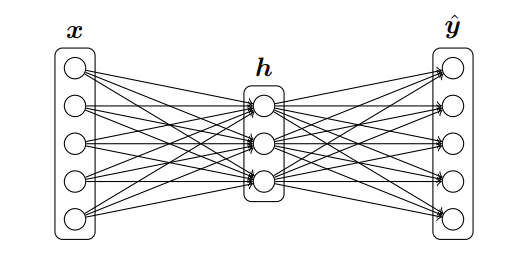
\includegraphics [scale=0.5] {FCNN}
	\caption{Neural Network} 
	\label{img:FCNN}  
\end{figure}

\noindent where $x$ is one-hot input vector, $h$ - hidden layer, y is the one-hot label vector, and ŷ is the predicted probability vector for all classes.The neural network Figure \ref{img:FCNN} employs sigmoid activation function for the hidden layer, and softmax for the output layer and cross entropy cost ~\ref{eq:equation2_7} is used.

\begin{equation}
\label{eq:equation2_8}
\textrm{CE}({\bf y},{\bf\hat{y}}) = -\sum_{i}{y_{i}\log{\hat{y_{i}}}}
	\end{equation}
\begin{doublespacing}
\end{doublespacing}

Now, we will compute the gradient of cross entropy:

\begin{equation}
\label{eq:equation_CE_2}
\frac{\partial(\textrm{CE})}{\partial{\hat{y}_{i}}} = -\frac{y_{j}}{\hat{y}_{i}}
	\end{equation}
\begin{doublespacing}
\end{doublespacing}
That leads, 

\begin{equation}
\frac{\partial(\textrm{CE})}{\partial{\theta_{k}}} =  \frac{\partial(\textrm{CE})}{\partial{\hat{y}_{i}}}\frac{\partial{\hat{y}_{i}}}{\partial{\theta_{k}}} 
=-\frac{y_{j}}{\hat{y}_{i}}\frac{\partial{\hat{y}_{i}}}{\partial{\theta_{k}}}
	\end{equation}
\begin{doublespacing}
\end{doublespacing}

Function $softmax$ for i-th output depends not only on its $\theta_{i}$, but also on all other $\theta_{k}$, the sum of which lies in the denominator of the formula for direct passage through the network. Therefore, the formula for back propagation "splits" into two: the partial derivative with respect to $\theta_{i}$ and $\theta_{k}$:

\begin{equation}
\begin{multlined}
\label{eq:equation_CE_3}
\frac{\partial{\hat{y}_{i}}}{\partial{\theta_{i}}} =  \frac{\partial}{\partial{\theta_{i}}}\left( \frac{e^{\theta_{i}}}{\sum_{j=1}{e^{\theta_{j}}}}\right) =\\
= \frac{e^{\theta_{i}}}{\sum_{j=1}{e^{\theta_{j}}}} - \left(\frac{e^{\theta_{i}}}{\sum_{j=1}{e^{\theta_{j}}}}\right)^{2} = \\
= \hat{y}_{i}\cdot(1 - \hat{y}_{i})
\end{multlined}
	\end{equation}
\begin{doublespacing}
\end{doublespacing}

and (where $i\neq k$),

\begin{equation}
\label{eq:equation_CE_4}
\begin{multlined}
\frac{\partial{\hat{y}_{i}}}{\partial{\theta_{k}}} =  \frac{\partial}{\partial{\theta_{k}}}\left( \frac{e^{\theta_{i}}}{\sum_{j=1}{e^{\theta_{j}}}}\right) = \\
=-\left(\frac{e^{\theta_{i}}e^{\theta_{k}}}{\sum_{j=1}{e^{\theta_{j}}}}\right)
= - \hat{y}_{i}\hat{y}_{k}
\end{multlined}
	\end{equation}
\begin{doublespacing}
\end{doublespacing}

After combination of equations~\ref{eq:equation_CE_2},~\ref{eq:equation_CE_3},~\ref{eq:equation_CE_4}, 

\begin{equation}
\label{eq:CE_gradient}
\frac{\partial(\textrm{CE})}{\partial{\theta_{k}}} = \begin{cases}
-y_{j}(1 - \hat{y}_{k})&\text{ for }i=k \\
y_{j}\hat{y}_{k}&\text{ for }i\neq k
\end{cases}
	\end{equation}
\begin{doublespacing}
\end{doublespacing}

$y_{j}$ should be non-zero, $k=j$ and $y_{j}=1$, leads to,

\begin{equation}
\label{eq:equation_CE_5}
\frac{\partial(\textrm{CE})}{\partial{\theta_{j}}} = \begin{cases}
(\hat{y}_{j} - 1)&\text{ for }i=j \\
\hat{y}_{j}&\text{ for }i\neq j
\end{cases}
	\end{equation}
\begin{doublespacing}
\end{doublespacing}

Which is equivalent to,

\begin{equation}
\frac{\partial(\textrm{CE})}{\partial{\boldsymbol\theta}} = \bf{\hat{y}} - \bf{y}
	\end{equation}
\begin{doublespacing}
\end{doublespacing}

\noindent Forward propagation is as follows:
\begin{equation}
{\bf h} = \textrm{sigmoid}({\bf x\textrm{W}_{1} + b_{1}}) 
	\end{equation}
\begin{doublespacing}
\end{doublespacing}

\begin{equation}
\label{eq:equation2_7}
{\bf \hat{y}} = \textrm{softmax}({\bf h\textrm{W}_{2} + b_{2})}
	\end{equation}
\begin{doublespacing}
\end{doublespacing}

\noindent where $\bf{\textrm{W}}_i$ and $\bf{b}_{i}$ ($i\in\{1,2\}$) are
the weights and biases, respectively of the two layers.
\indent To optimize weights for each layer of neural network a back propagation algorithm is used. Therefore, it is necessary to calculate the gradients for each layer.
  
\noindent In order to simplify the notation used to solve the problem, define the following terms:
\begin{equation}
\label{eq:equation2_10}
\begin{multlined}
		 {\bf z}_{1}\equiv \quad{\bf x\textrm{W}_{1} + b_{1}} \\
		{\bf z}_{2}\equiv \quad{\bf h\textrm{W}_{2} + b_{2}}
\end{multlined}
	\end{equation}
\begin{doublespacing}
\end{doublespacing}
Starting with the results from ~\ref{eq:equation2_8}:

\begin{equation}
\frac{\partial{J}}{\partial{\bf z}_{2}} = \bf{\hat{y}} - \bf{y}
\end{equation}
and

\begin{equation}
\label{eq:equation2_11}
\frac{\partial{\bf z}_{2}}{\partial{{\bf h}}} = {\bf \textrm{W}^{\top}_{2}}
\end{equation}
Sigmoid ($\sigma$) derivative ~\ref{eq:equation2_6}:

\begin{equation}
\frac{\partial{{\bf h}}}{\partial{{\bf z}_{1}}}\equiv\sigma^{\prime}(z_{1})
\end{equation}
Combining these, and using $\cdot$ to denote element-wise product:

\begin{equation}
\frac{\partial{J}}{\partial{z_{i}}} = (\bf{\hat{y}} - \bf{y}){\bf \textrm{W}^{\top}_{2}}\cdot\sigma^{\prime}(z_{1})
\end{equation}
Finally, using the results from Equation~\ref{eq:equation2_11}:

\begin{equation}
\frac{\partial{J}}{\partial{{\bf W}^{(1)}}} = (\bf{\hat{y}} - \bf{y}){\bf \textrm{W}^{\top}_{2}}\cdot\sigma^{\prime}(z_{1})\cdot{\bf \textrm{X}^{\top}}
\end{equation}  

\begin{equation}
\frac{\partial{J}}{\partial{{\bf W}^{(2)}}} = (\bf{\hat{y}} - \bf{y}){\bf \textrm{h}^{\top}}
	\end{equation}
\begin{doublespacing}
\end{doublespacing}  
We have everything to update our weights: 
Now, turn definitely to skip-gram model shown in Figure ~\ref{img:skip_gram_model}\cite{embeddings_2}:
\begin{figure}[H] 
	\center
	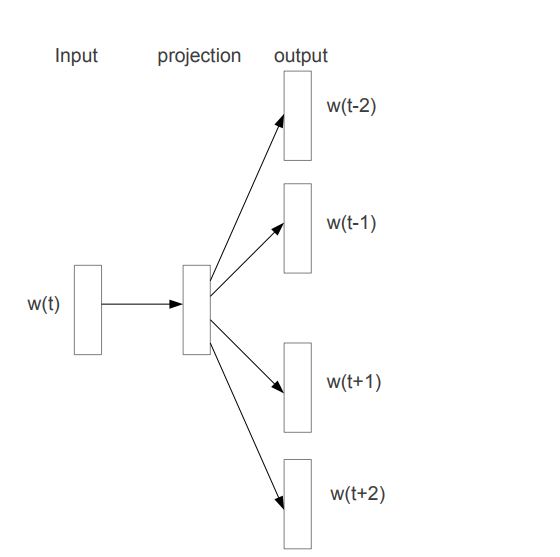
\includegraphics [scale=0.5] {skip_gram_model}
	\caption{The Skip-gram model architecture.} 
	\label{img:skip_gram_model}  
\end{figure}



\noindent Now, let`s transfer knowledge from above to our skip-gram model.    
We have a word vector ${\boldsymbol v}_{c}$ corresponding to the center word $c$ for
\texttt{skip-gram}, and word prediction is made with the \texttt{softmax} function: 

\begin{equation}
{\hat{\boldsymbol y}}_{\boldsymbol o} = p(~{\boldsymbol o} \mid {\boldsymbol c}~) = \frac{\exp{({\boldsymbol u}^{\top}_{o}{\boldsymbol v}_{c})}}{\sum^{\vert{W}\vert}_{j=1}\exp{({\boldsymbol u}^{\top}_{j}{\boldsymbol v}_{c})}}
	\end{equation}
\begin{doublespacing}
\end{doublespacing}
where $w$ denotes the $w$-th word and ${\boldsymbol u}_{w}$ ($w=1,...,\vert\textrm{W}\vert$)  are the `output' word vectors for all words in the vocabulary. Cross entropy cost is applied to this prediction and word $o$ is the expected word (the $o$-th element of the one-hot label vector is one). ${\boldsymbol U} = [ {\boldsymbol u}_{1}, {\boldsymbol u}_{2},...,{\boldsymbol u}_{\vert\textrm{W}\vert}]$ is the matrix of all the output vectors. 
Applying cross-entropy cost to the softmax probability defined above:

\begin{equation}
J =-\log{p} = - {\boldsymbol u}_{o}^{\top}{\boldsymbol v}_{c} + \log\sum^{\vert{V}\vert}_{j=1}\exp{({\boldsymbol u}_{j}^{\top}{\boldsymbol v}_{c})}
	\end{equation}
\begin{doublespacing}
\end{doublespacing}
Let $z_{j}={\boldsymbol u}_{j}^{\top}{\boldsymbol v}_{c}$, and $\delta^{i}_{j}$ ~\ref{eq:indicator} be the indicator function, then

\begin{equation}
\label{eq:indicator}
\delta^{i}_{j} =  
	\begin{cases}
	1, &\text{ for }i=j \\
	0, &\text{ for }i\neq j
	\end{cases}
	\end{equation}
\begin{doublespacing}
\end{doublespacing}


\begin{equation}
\frac{\partial J}{\partial{z_{k}}} = - \delta^{i}_{k} + \frac{\exp{({\boldsymbol u}_{i}^{\top}{\boldsymbol v}_{c})}}{\sum^{\vert{V}\vert}_{j=1}\exp{({\boldsymbol u}_{j}^{\top}{\boldsymbol v}_{c})}}
	\end{equation}
\begin{doublespacing}
\end{doublespacing}
Now, using the chain rule, we can calculate,

\begin{equation}
	\begin{multlined}
	\frac{\partial J}{\partial{{\boldsymbol v}_{c}}} =  \frac{\partial J}{\partial{{\boldsymbol z}}}\frac{\partial{{\boldsymbol z}}}{\partial{{\boldsymbol v}_{c}}} =\\
	= \sum^{\vert{V}\vert}_{j=1}{\boldsymbol u}_{j}^{\top}\left(\frac{e^{z_{j}}}{\sum^{\vert{V}\vert}_{k=1}e^{z_{k}}} -  1\right) =\\
	= \sum^{\vert{V}\vert}_{k=1}{\boldsymbol P}({\boldsymbol u}_{j} \vert {\boldsymbol v}_{c} ){\boldsymbol u}_{j} - {\boldsymbol u}_{j}
	\end{multlined}
	\end{equation}
\begin{doublespacing}
\end{doublespacing}

\noindent For the `output' word vectors ${\boldsymbol u}_{w}$'s

\begin{equation}
	\begin{multlined}
	\frac{\partial J}{\partial{\boldsymbol u}_{j}} = \frac{\partial J}{\partial{{\boldsymbol z}}}\frac{\partial{{\boldsymbol z}}}{\partial{\boldsymbol u}_{j}} =\\
	= {\boldsymbol v}_{c}\left(\frac{\exp{({\boldsymbol u}^{\top}_{0}{\boldsymbol v}_{c})}}{\sum^{\vert{V}\vert}_{j=1}\exp{({\boldsymbol u}^{\top}_{j}{\boldsymbol v}_{c})}} - \delta^{0}_{j}\right)
	\end{multlined}
	\end{equation}
\begin{doublespacing}
\end{doublespacing}

\noindent We have calculated the gradient for one particular word, now we will generalize this to a number of words. We have a set of context words [$\texttt{word}_{c-\textbf{m}},...,\texttt{word}_{c-\textbf{1}},\texttt{word}_{c},\texttt{word}_{c+\textbf{1}},...,\texttt{word}_{c+\textbf{m}}$ ], where \textbf{m} is the context size. We denote the `input' and `output' word vectors for $\texttt{word}_{k}$ as ${\boldsymbol v}_{k}$ and ${\boldsymbol u}_{k}$ respectively for
convenience. \\

\noindent Also it is a good idea to use $F({\boldsymbol o}, {\boldsymbol v}_{c})$ (where ${\boldsymbol o}$ is the expected word) as a placeholder for $J({\boldsymbol o}, {\boldsymbol v}_{c}, ...)$ cost functions.

\noindent Then we can rewrite cost function as follows:

\begin{equation}
J =   \sum_{-m\le j\le m, j\neq0}F({\boldsymbol w}_{c+j}, {\boldsymbol v}_{c})
	\end{equation}
\begin{doublespacing}
\end{doublespacing}
where ${\boldsymbol w}_{c+j}$ refers to the word at the $j$-th index from the center.\\

The derivative of the loss has two terms, ${\boldsymbol w}_{c+j}$ and ${\boldsymbol v}_{c}$, which yields the following ~\cite{assignment1},

\begin{equation}
	\begin{multlined}
	\frac{\partial{J}}{\partial{\boldsymbol w}_{k}} = \\ =\frac{\partial}{\partial{\boldsymbol w}_{k}}\sum_{-m\le j\le m, j\neq0}F({\boldsymbol w}_{c+j}, {\boldsymbol v}_{c})= \\
	= \sum_{-m\le j\le m, j\neq0} \frac{\partial{F}}{\partial{\boldsymbol w}_{i+j}}\delta^{i+j}_{k}
	\end{multlined}
	\end{equation}
\begin{doublespacing}
\end{doublespacing}
and

\begin{equation}
\frac{\partial{J}}{\partial{\boldsymbol v}_{c}} = \sum_{-m\le j\le m, j\neq0} \frac{\partial{F}}{\partial{\boldsymbol v}_{c}}
	\end{equation}
\begin{doublespacing}
\end{doublespacing}
Now, we can update our weight using gradient descent algorithm:

\begin{equation}\\
	\begin{multlined}
	w^{new}_{k} = w^{old}_{k} - \eta \frac{\partial{J}}{\partial{w}_{k}} \\
	v^{new}_{c} = v^{old}_{c} - \eta \frac{\partial{J}}{\partial{v}_{c}}
	\end{multlined}
	\end{equation}
\begin{doublespacing}
\end{doublespacing}
where $\eta$ is a learning rate.

After training the skip-gram model, we take the hidden layer weight matrix that will represent our words in the multidimensional space. If we make projection into two- dimensional space, we can have the following Figure ~\ref{img:embed}:

\begin{figure}[ht] 
	\center
	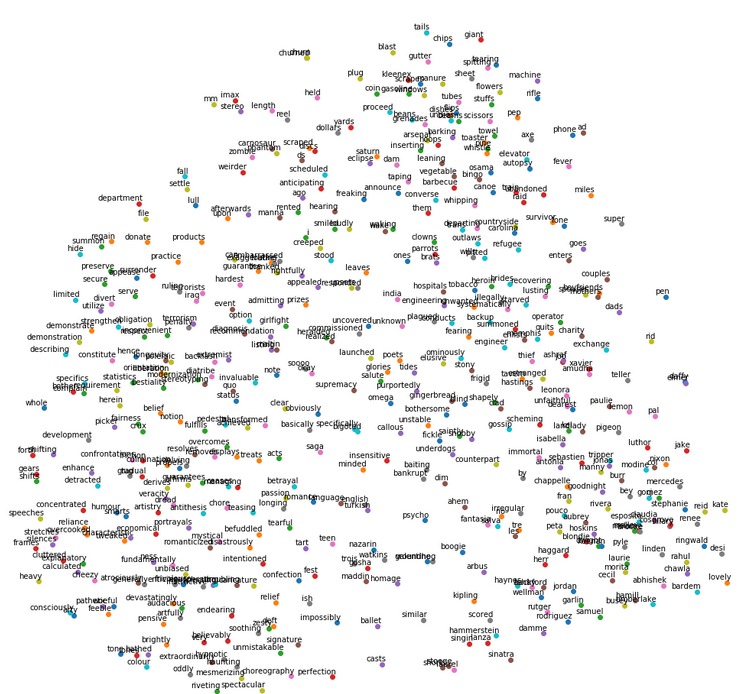
\includegraphics [scale=0.4] {embed}
	\caption{Words representation} 
	\label{img:embed}  
\end{figure}


However, this type of architecture, where for each output we need to compute separate $softmax$ function is very expensive in terms of computational resources and as a result time. Therefore, there are different ways to approximate the expensive $softmax$ function. The most famous of them are:

\begin{itemize}
	\item Negative Sampling technique
	\item Hierarchical Softmax
\end{itemize}
 

\noindent The only difference between Negative Sampling technique and the original model is that we introduce new loss function - negative sampling loss for the predicted vector ${\boldsymbol v}_{c}$, and 
the expected output word is ${\boldsymbol o}({\boldsymbol u}_{o})$. Assume that $K$ negative samples (words) are drawn, and they are ${\boldsymbol u}_{1},...,{\boldsymbol u}_{k}$, respectively for simplicity of notation ($k\in\{1,...,K\}$ and $o\notin\{1,...,K\}$). Again for a given word, ${\boldsymbol o}$, denote its output vector as ${\boldsymbol u}_{o}$. The negative sampling loss function in this case is,

\begin{equation}
J({\boldsymbol u}_{o}, {\boldsymbol v}_{c}, {\boldsymbol U}) = -\log(\sigma( {\boldsymbol u}^{\top}_{o}{\boldsymbol v}_{c})) - \sum^{K}_{k=1}\log(\sigma(- {\boldsymbol u}^{\top}_{k}{\boldsymbol v}_{c}))
	\end{equation}
\begin{doublespacing}
\end{doublespacing}
where $\sigma(\cdot)$ is the sigmoid function.\\
As it can be clearly seen, now we make calculations not on the whole vocabulary $V$, but only on the part of it, which is randomly generated each time. 

~\\ 
Hierarchical Softmax is an approximation which uses a binary tree to compute the necessary probability. 
This gives us a possibility to decompose calculating the probability of one word into a sequence of probability calculations. Balanced threes have a maximum depth of $log_2(|V|)$, which means that in the worst case we need to calculate $log_2(|V|)$ nodes to find the necessary probability of a certain word.  

Both methods enable us a possibility to significantly decrease the amount of time for computation.

2.CBOW model
This model is very similar to skip-gram, but CBOW predicts a target word from the bag of words context. From the practical point of view, skip-gram works well with a small amount of training data and represents well even rare words or phrases. CBOW is several times faster to train than the skip-gram and has slightly better accuracy for the frequent words. This model is shown in Figure ~\ref{img:CBOW}\cite{embeddings_2}:

\begin{figure}[ht] 
	\center
	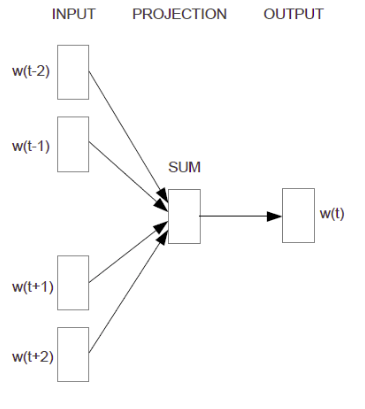
\includegraphics [scale=0.6] {CBOW}
	\caption{The CBOW model architecture.} 
	\label{img:CBOW}  
\end{figure}

\section{Deep learning algorithms for text classification}\label{sect2_2}

When people hear about NLP problems and neural networks in one context they probably think about Recurrent neural networks or their modification. 
However, recently some papers which apply CNN's to problems in Natural Language Processing were published and they got some interesting results \cite{CNN} \cite{Kalchbrenner}. In this section I will consider both CNN and RNN models and their modifications.


\subsection{Convolution Neural Networks}\label{sect2_2_1}  

\begin{figure}[ht] 
	\center
	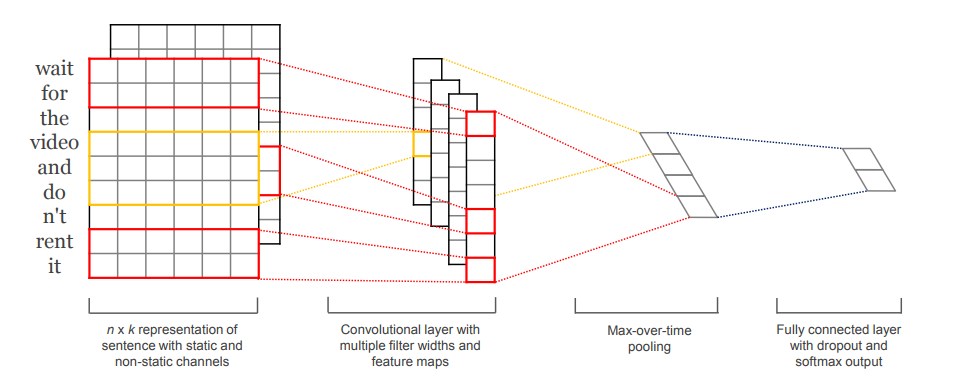
\includegraphics [scale=0.5] {CNN}
	\caption{Convolution Neural Networks architecture for text classification} 
	\label{img:CNN}  
\end{figure}

The model architecture, shown in Figure ~\ref{img:CNN} \cite{CNN}, is a variant of the CNN architecture. Let $x_i \in \mathbb{X}$ be the k-dimensional word vector corresponding to the i-th word in the sentence, a sentence of length n. In general, let $x_{i:i+j}$ refers to the concatenation of words $\{x_{i}, x_{i+1}, . . . , x_{i+j}\}$.\cite{CNN}


\subsubsection{Convolution}\label{sect2_2_1_1} 

\begin{figure}[ht] 
	\center
	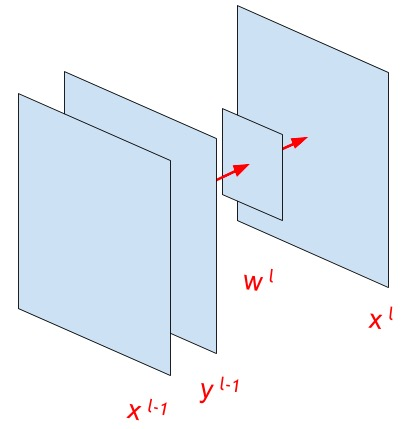
\includegraphics [scale=0.5] {convolution}
	\caption{Basic variables used in the convolution layer} 
	\label{img:convolution}  
\end{figure}

In the convolution neural network, a limited matrix of small weights is used in the convolution operation, which is moved along the entire processed layer, forming after each shift the activation signal for the neuron of the next layer with the same position. The same matrix of weights, called kernel, is used for different neurons of the output layer.  
The schema of this process is illustrated in the Figure ~\ref{img:convolution} \cite{CNN_habr}.

The following equation ~\ref{eq:convolution} describes the words above into mathematical way:

\begin{equation}
\label{eq:convolution}
x^l_{ij}=\sum_{a=-\infty}^{+\infty}\sum_{b=-\infty}^{+\infty}w^l_{ab}\cdot y^{l-1}_{(i\cdot s-a)(j\cdot s-b)}+b^l \qquad \forall i\in (0,...,N) \enspace \forall j\in (0,...,M) 
	\end{equation}
\begin{doublespacing}
\end{doublespacing}
where $i, j, a, b$ - indexes of elements in matrices, $s$ - step's size of convolution

\noindent The superscripts $l$ and $l-1$ are the indices of the network layers.\\
$x_{l-1}$ - the output of some previous function, or the input of the network \\
$y_{l-1}$ - $x_{l-1}$ after passing the activation function \\
$w_{l}$ - the convolution kernel \\
$b_{l}$ - bias or offset \\
$x_{l}$ - the result of the operation of convolution. That is, the operations which goe separately for each element $i,j$ of the matrix $x_{l}$, whose dimension is $(N, M)$.

The important moment which I should pay attention to is Central Core Element, because indexing of the elements takes place depending on the location of the central element. In fact, the central element determines the origin of the "coordinate axis" of the convolution kernel. 

\subsubsection{Activation functions}
\indent Activation function is a transformation which has a general view $y^l=f(x^l)$. I did not cover all existing activations functions, I chose only those which were used in the current model. 

1) ReLu \ref{eq:Relu}, \ref{img:Relu} - this activation function was used at Convolution layers. It has the following properties:


\begin{equation}
\label{eq:Relu}
f_{ReLU}=max(0,x)
	\end{equation}
\begin{doublespacing}
\end{doublespacing}

\begin{figure}[H] 
	\center
	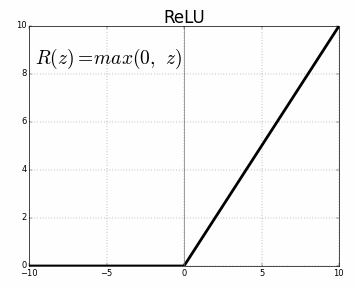
\includegraphics [scale=0.4] {Relu}
	\caption{ReLu activation function} 
	\label{img:Relu}  
\end{figure}


2) Softmax \ref{eq:equation2_4} - I deal with multi-class classification, therefore this activation was picked.


\subsubsection{Max pulling layer} 
\indent This layer allows one to highlight important features on the maps of features obtained from convolution layer, gives an invariance to find the object on the cards, and also reduces the dimensionality of the maps, speeding up the network time. It works in the following way Figure \ref{img:max_pulling}: we divide our features from convolution layer into disjoint $m \times n$ regions, and take the maximum feature activation over these regions. These new features can be used for classification.

\begin{figure}[ht] 
	\center
	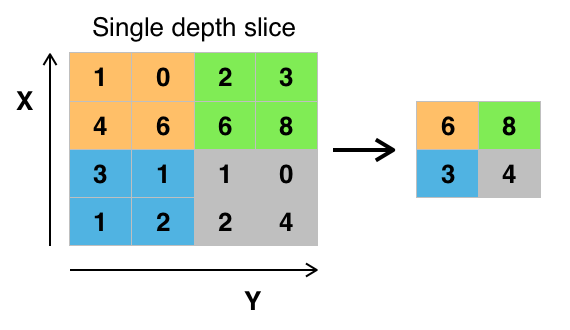
\includegraphics [scale=0.5]{max_pulling}
	\caption{Max pulling layer} 
	\label{img:max_pulling}  
\end{figure}


\subsubsection{Fully connected layer}
\indent After layers of the convolution and max pooling, we obtain a set of feature cards. We connect them into one vector and this vector will be fed into the fully connected network.
The Figure \ref{img:CNN_FNN_layer} describes this stage.

\begin{figure}[ht] 
	\center
	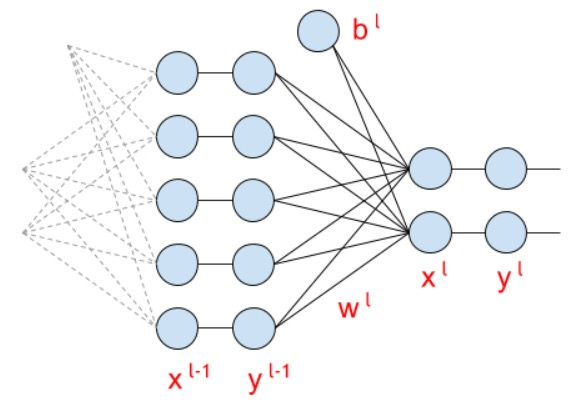
\includegraphics [scale=0.5] {CNN_FNN_layer}
	\caption{Fully connected layer of CNN} 
	\label{img:CNN_FNN_layer}  
\end{figure}

\begin{equation}
x^l_i=\sum_{k=0}^{m}w^l_{ki}y^{l-1}_k+b^l_i \qquad \forall i\in (0,...,n)
	\end{equation}
\begin{doublespacing}
\end{doublespacing}
in matrix representation:

\begin{equation}
	X^l=Y^{l-1}W^l+B^l_i 
	\end{equation}
\begin{doublespacing}
\end{doublespacing}
\noindent Loss function for the model is Cross Entropy \ref{eq:equation2_8} described above.

Now after all components of CNN are known, we need to optimize weights for each layer. Therefore, it is necessary to derive the formula for back propagation through the loss function. 

1) Hopefully, the gradient for loss function was already founded \ref{eq:equation_CE_3}, \ref{eq:equation_CE_4}, \ref{eq:CE_gradient}.
Therefore, we have the following equation \ref{eq:CNN_softmax_grad}: 

\begin{equation}
	\label{eq:CNN_softmax_grad}
	\begin{multlined}
	 \frac{\partial J}{\partial x^l_i} = \sum_{k=0}^{n} \frac{\partial J}{\partial y^l_k} \frac {\partial y^l_k} {\partial x^l_i} = \frac{\partial J}{\partial y^l_0} \frac {\partial y^l_0} {\partial x^l_i} + ... \\ + \frac{\partial J}{\partial y^l_1} \frac {\partial y^l_1} {\partial x^l_i} + ...
	 + \frac{\partial J}{\partial y^l_n} \frac {\partial y^l_n} {\partial x^l_i} \qquad \forall i \in (0,...n)
	\end{multlined}
	\end{equation}
\begin{doublespacing}
\end{doublespacing}
or 
\begin{equation}
\label{eq:CNN_softmax_grad_long}
	\begin{multlined}
	\begin{bmatrix} 
	&\frac{\partial J}{\partial x^{l}_{0}} &\frac{\partial J}{\partial x^{l}_{1}} & ... &\frac{\partial J}{\partial x^{l}_{n}} 
	\end{bmatrix} 
	= \\= \scriptsize 
	\begin{bmatrix} & (\frac{\partial J}{\partial y^{l}_{0}}\frac{\partial y^{l}_{0}}{\partial x^{l}_{0}}+\frac{\partial J}{\partial y^{l}_{1}}\frac{\partial y^{l}_{1}}{\partial x^{l}_{0}}+\ldots+\frac{\partial J}{\partial y^{l}_{n}}\frac{\partial y^{l}_{n}}{\partial x^{l}_{0}}) & (\frac{\partial J}{\partial y^{l}_{0}}\frac{\partial y^{l}_{0}}{\partial x^{l}_{1}}+\frac{\partial J}{\partial y^{l}_{1}}\frac{\partial y^{l}_{1}}{\partial x^{l}_{1}}+\ldots+\frac{\partial J}{\partial y^{l}_{n}}\frac{\partial y^{l}_{n}}{\partial x^{l}_{1}}) & ... & (\frac{\partial J}{\partial y^{l}_{0}}\frac{\partial y^{l}_{0}}{\partial x^{l}_{n}}+\frac{\partial J}{\partial y^{l}_{1}}\frac{\partial y^{l}_{1}}{\partial x^{l}_{n}}+\ldots+\frac{\partial J}{\partial y^{l}_{n}}\frac{\partial y^{l}_{n}}{\partial x^{l}_{n}}) 
	\end{bmatrix} \\= 
	\begin{bmatrix} &\frac{\partial J}{\partial y^{l}_{0}} &\frac{\partial J}{\partial y^{l}_{1}} & ... &\frac{\partial J}{\partial y^{l}_{n}} 
	\end{bmatrix} 
	\begin{bmatrix} &\frac{\partial y^{l}_{0}}{\partial x^{l}_{0}} &\frac{\partial y^{l}_{0}}{\partial x^{l}_{1}}&...&\frac{\partial y^{l}_{0}}{\partial x^{l}_{n}}\\ &\frac{\partial y^{l}_{1}}{\partial x^{l}_{0}} &\frac{\partial y^{l}_{1}}{\partial x^{l}_{1}}&...&\frac{\partial y^{l}_{1}}{\partial x^{l}_{n}}\\ &...&...&...&...\\ &\frac{\partial y^{l}_{n}}{\partial x^{l}_{0}} &\frac{\partial y^{l}_{n}}{\partial x^{l}_{1}}&...&\frac{\partial y^{l}_{n}}{\partial x^{l}_{n}}\\ 
	\end{bmatrix}
	\end{multlined}
	\end{equation}
\begin{doublespacing}
\end{doublespacing}
Next, we should update the weights of fully connected layer matrix $w^l$. 
\begin{equation}
\frac{\partial J}{\partial w^l} = \dfrac{\partial J}{\partial y^l}\dfrac{\partial y^l}{\partial x^l}\dfrac{\partial x^l}{\partial w^l} = \delta^l \cdot \dfrac{\partial x^l}{\partial w^l} = \left(y^{l-1} \right)^T \cdot \delta^l    
	\end{equation}
\begin{doublespacing}
\end{doublespacing}
and $b^l$

\begin{equation}
\frac{\partial J}{\partial b^l}=\delta^l
	\end{equation}
\begin{doublespacing}
\end{doublespacing}
Equation for back propagation through $y^{l-1}$

\begin{equation}
 \dfrac{\partial J}{\partial y^{l-1}} = \delta^l \cdot \dfrac{\partial x^l}{\partial y^{l-1}}= \delta^l \cdot (w^l)^{T} = \delta^{l-1}
	\end{equation}
\begin{doublespacing}
\end{doublespacing} 

After this, we need to go with backprop through the layer of max pulling Figure \ref{img:backprog_max_pulling}.
The error "passes" only through those values of the original matrix, which were chosen by the maximum at the step of the max puling. The remaining error values for the matrix will be zero. 

\begin{figure}[ht] 
	\center
	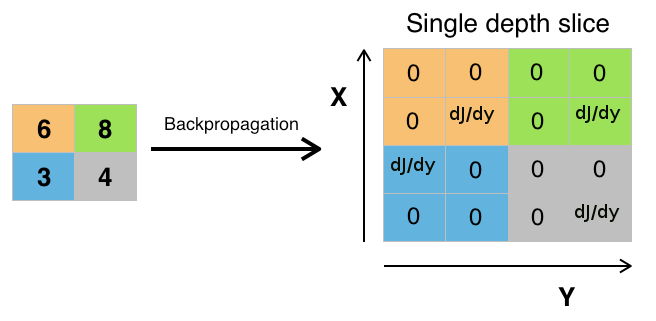
\includegraphics [scale=0.5]{backprog_max_pulling}
	\caption{Back propagation through max pulling layer} 
	\label{img:backprog_max_pulling}  
\end{figure}
It is necessary to derive weights update for kernel Figure \ref{img:conv_grad}. 

\begin{figure}[ht] 
	\center
	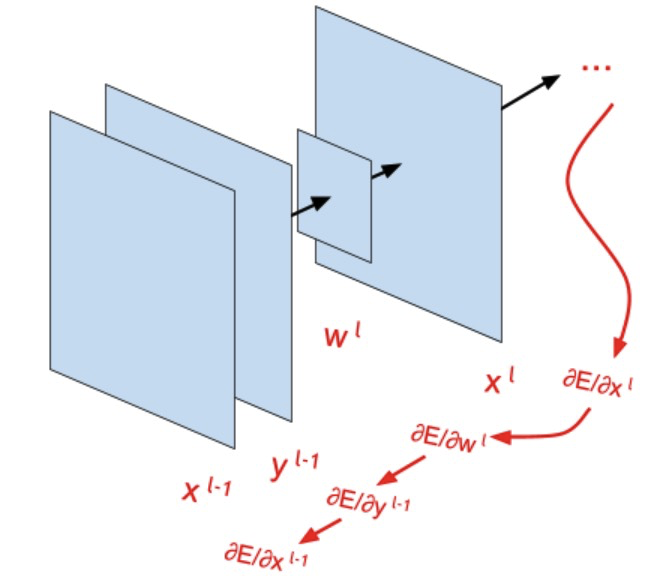
\includegraphics [scale=0.4]{conv_grad}
	\caption{Back propagation through convolution layer} 
	\label{img:conv_grad}  
\end{figure}

\begin{equation}
\begin{array}{rcl} 
\dfrac{\partial J}{\partial w^l_{ab}}&=&\sum_{i}\sum_{j} \dfrac{\partial J}{\partial y^l_{ij}}\dfrac{\partial y^l_{ij}}{\partial x^l_{ij}}\dfrac{\partial x^l_{ij}}{\partial w^l_{ab}}\\ &=&^{(1)}\sum_{i}\sum_{j} \dfrac{\partial J}{\partial y^l_{ij}}\dfrac{\partial y^l_{ij}}{\partial x^l_{ij}}\cdot \dfrac{\partial \left( \sum_{a'=-\infty}^{+\infty} \sum_{b'=-\infty}^{+\infty} w^l_{a'b'} \cdot y^{l-1}_{(is-a')(js-b')}+b^l \right)}{\partial w^l_{ab}}\\ &=&^{(2)}\sum_{i}\sum_{j} \dfrac{\partial J}{\partial y^l_{ij}}\dfrac{\partial y^l_{ij}}{\partial x^l_{ij}} \cdot y^{l-1}_{(is-a)(js-b)} \\ &&\forall a \in (-\infty,...,+\infty) \enspace \forall b \in (-\infty,...,+\infty) 
\end{array}\\
	\end{equation}
\begin{doublespacing}
\end{doublespacing}
all partial derivatives in the numerator, except those for which $a^{'}= a, b^{'} = b$, will be zero. 

~\\
Derivation of the gradient for the bias element. 
\begin{equation}
 \dfrac{\partial J}{\partial b^l} = \sum_{i}\sum_{j} \dfrac{\partial J}{\partial y^l_{ij}}\dfrac{\partial y^l_{ij}}{\partial x^l_{ij}}\dfrac{\partial x^l_{ij}}{\partial b^l} = \sum_{i}\sum_{j} \dfrac{\partial J}{\partial y^l_{ij}}\dfrac{\partial y^l_{ij}}{\partial x^l_{ij}} 
	\end{equation}
\begin{doublespacing}
\end{doublespacing}
\noindent The derivation of the equation for backprop through the convolution layer.

\begin{equation}
\frac{\partial J}{\partial y^{l-1}_{ij}}= \sum_{i'}\sum_{j'} \frac{\partial J}{\partial y^l_{i'j'}}\frac{\partial y^l_{i'j'}}{\partial x^l_{i'j'}} \cdot w^{l}_{(i-i's)(j-j's)}
	\end{equation}
\begin{doublespacing}
\end{doublespacing}

\subsection{Recurrent neural networks and their modifications} 
A recurrent neural network (RNN) is a class of artificial neural network where connections between units form a directed graph along a sequence. This allows it to exhibit dynamic temporal behavior for a time sequence. Unlike feedforward neural networks, RNNs can use their internal state (memory) to process sequences of inputs. This makes them applicable to such tasks as natural language processing. \cite{wiki_def_rnn}
Recurrent neural networks are networks with loops in them, allowing information to persist.
Figure \ref{img:rnn_structure} \cite{colah_lstm} illustrates RNN where, $A$ looks at some input $x_t$ and outputs a value $h_t$. $A$ loop allows information to pass from one step of the network to the next.

\begin{figure}[ht] 
	\center
	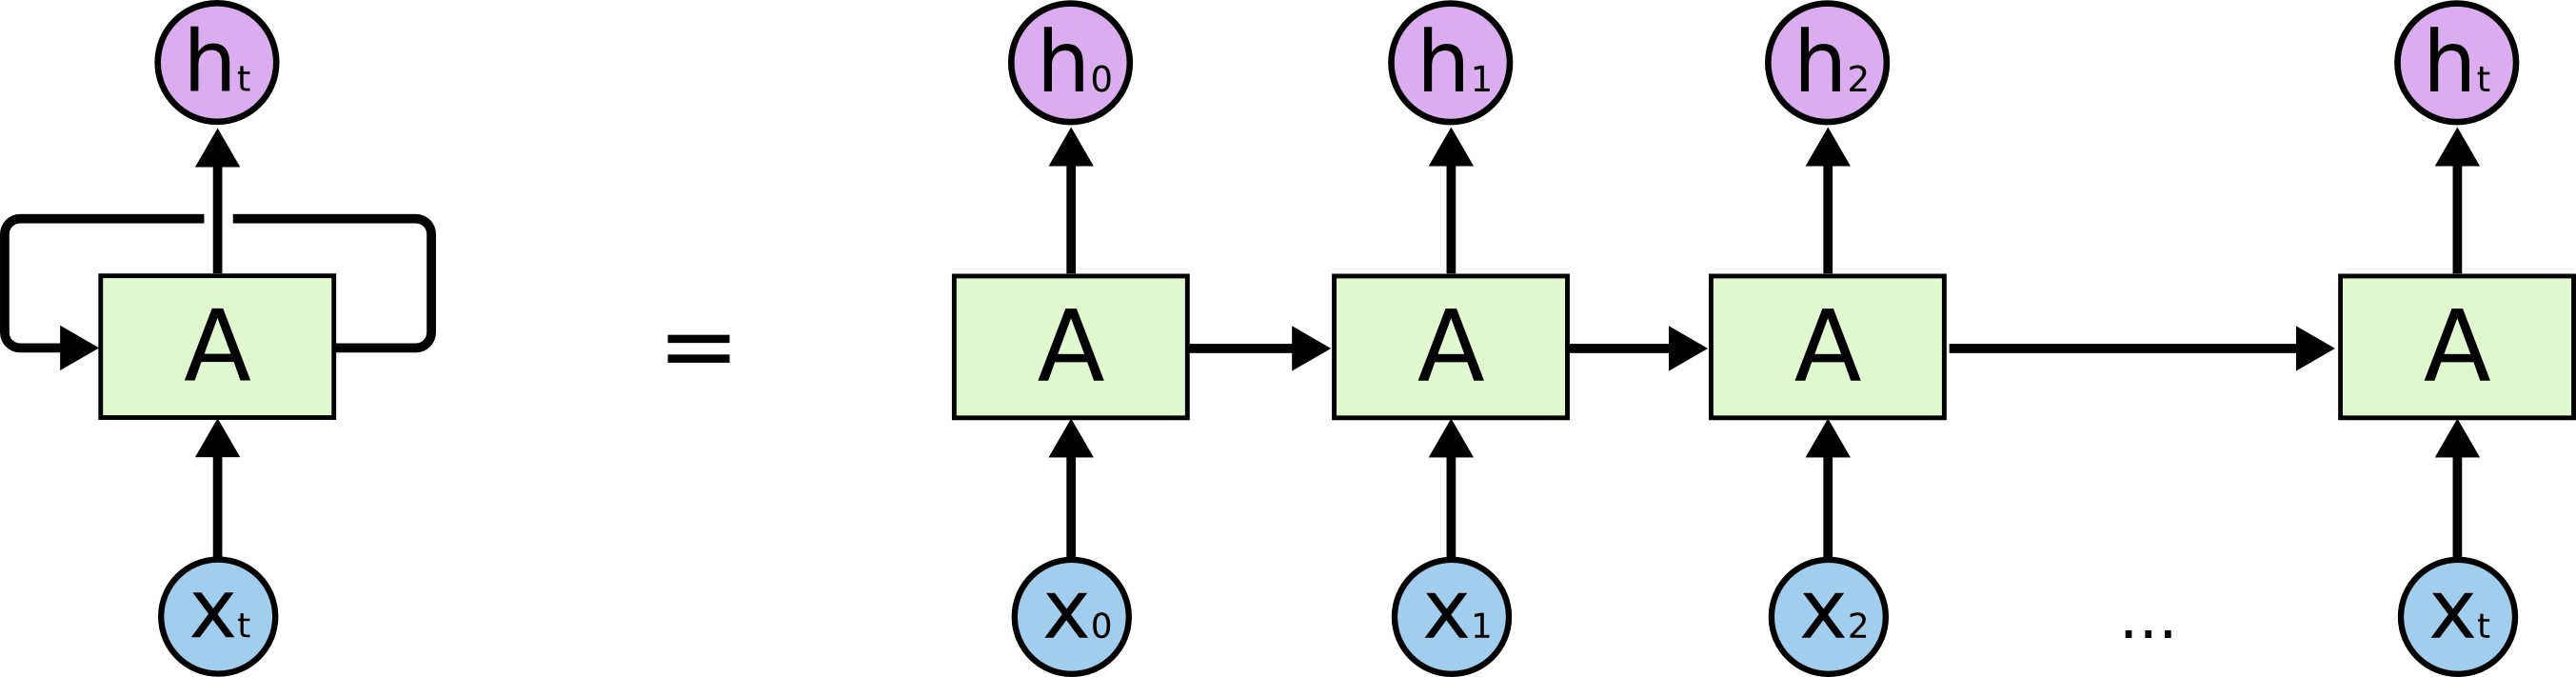
\includegraphics [scale=0.4]{rnn_structure}
	\caption{The structure of Recurrent neural network} 
	\label{img:rnn_structure}  
\end{figure}

However, this type of NN has problems called "Vanishing Gradient and Gradient Explosion Problems". 
This problem was studied in detail in \cite{rnn_problems}. Therefore, the most successful for 
practical issues are modified RNN. I will use the most popular type - Long Short Term Memory networks.

LSTMs are explicitly designed to avoid the long-term dependency problem. Remembering information for long periods of time is practically their default behavior. This features is achieved by more complex structure.
We can compare both architectures in Figure \ref{img:SimpleRNN}\cite{colah_lstm} and Figure \ref{img:LSTM}\cite{colah_lstm}.

\begin{figure}[ht] 
	\center
	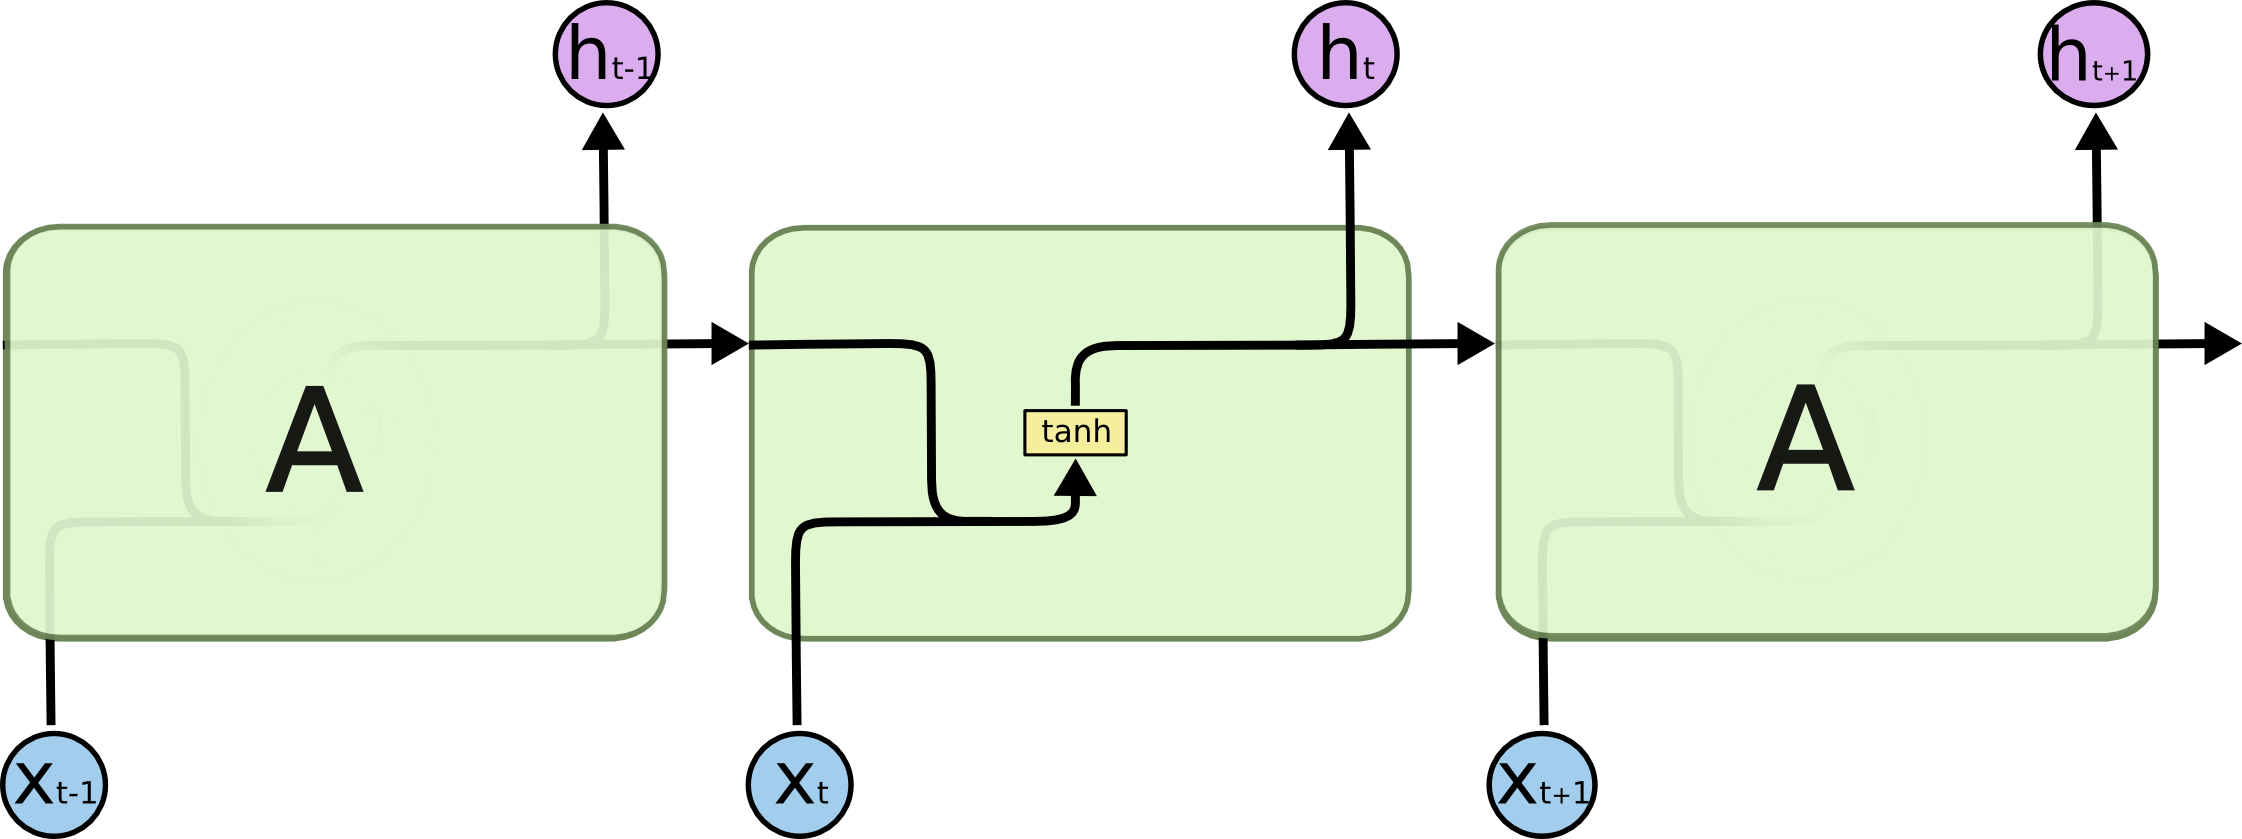
\includegraphics [scale=0.4]{SimpleRNN}
	\caption{The architecture of Recurrent neural network} 
	\label{img:SimpleRNN}  
\end{figure} 

\begin{figure}[ht] 
	\center
	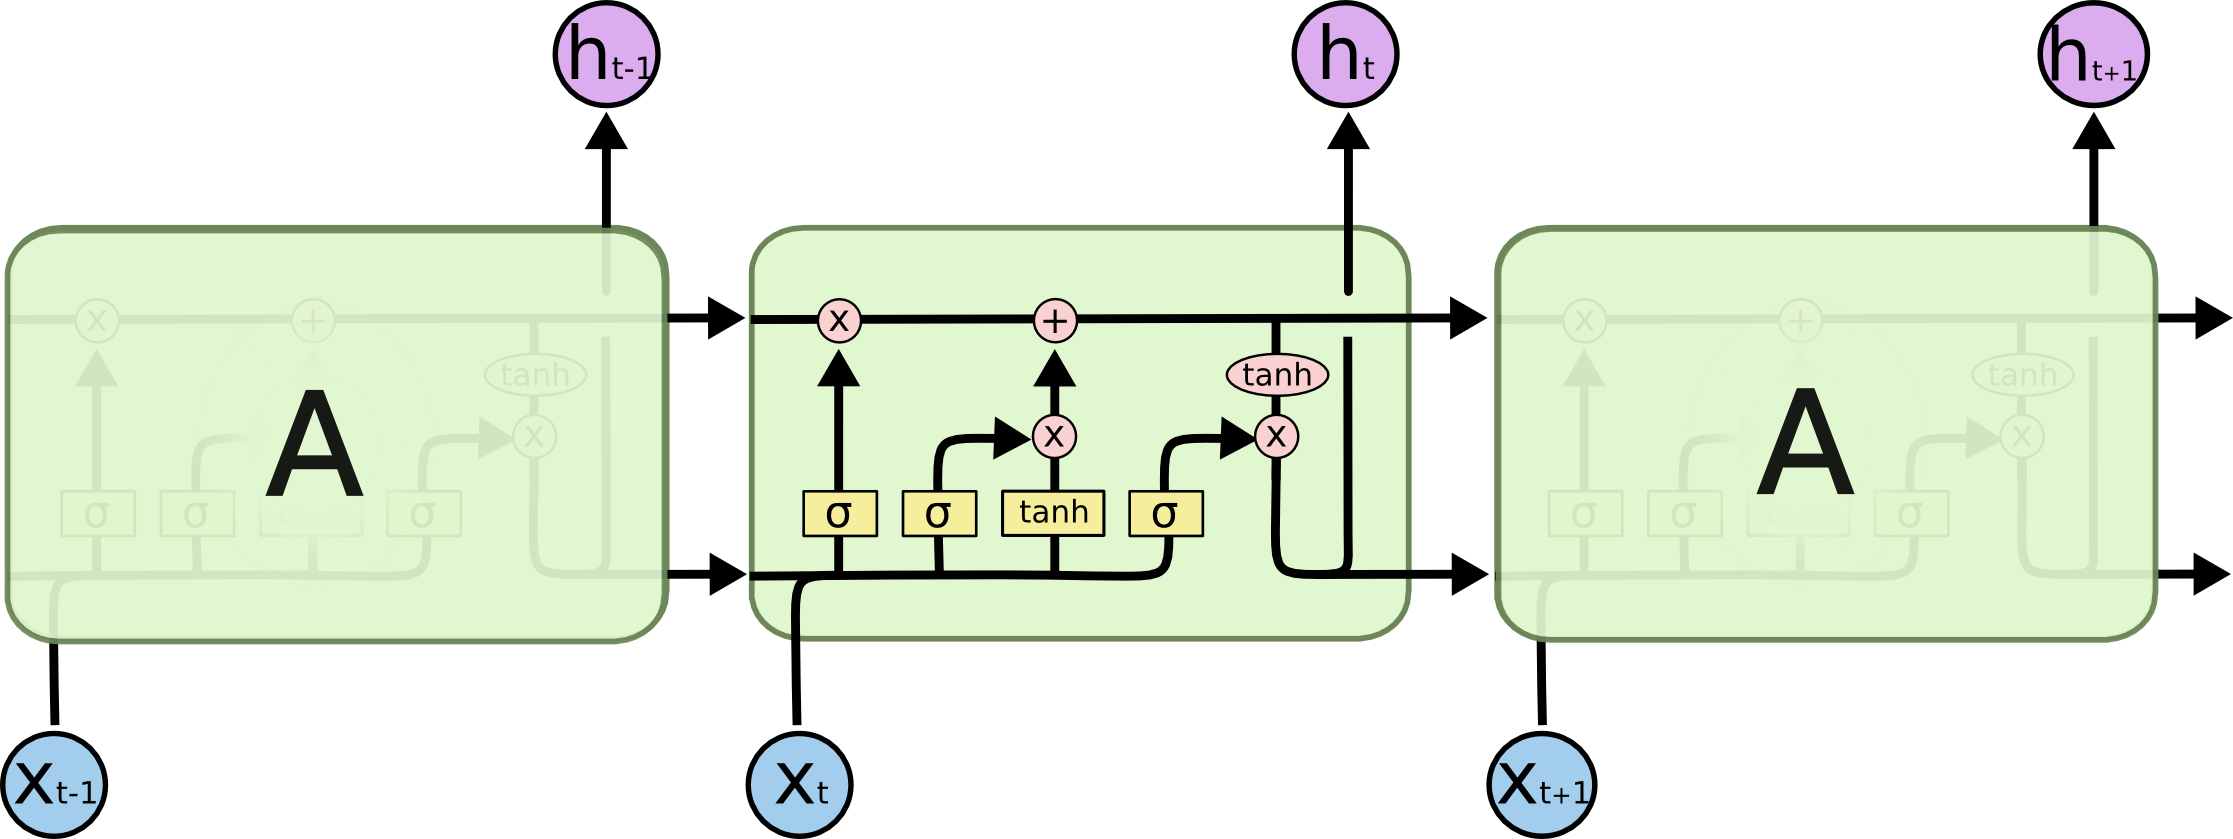
\includegraphics [scale=0.4]{LSTM}
	\caption{The architecture of Long Short Term Memory neural network} 
	\label{img:LSTM}  
\end{figure} 

The first step in LSTM is to decide what information we are going to throw away from the cell state. This decision is 
made by a sigmoid layer called the forget gate layer which 
looks at $h_{t-1}$ and $x_t$, and outputs a number between 0 
and 1 for each number in the cell state $C_{t-1}$.

\begin{equation}
f_t = \sigma(W_f[h_{t-1}, x_t] + b_f)
	\end{equation}
\begin{doublespacing}
\end{doublespacing}

The next step is to decide what new information we’re going to store in the cell state. This has two parts. First, a sigmoid layer called the input gate layer decides which values we’ll update. Next, a $tanh$ layer creates a vector of new candidate values, $\tilde{C}_t$, that could be added to the state. In the next step, we combine these two to create an update to the state.

\begin{equation}
i_t = \sigma(W_i[h_{t-1}, x_t] + b_i)
	\end{equation}
\begin{doublespacing}
\end{doublespacing}

\begin{equation}
\tilde{C}_t = \tanh(W_C[h_{t-1}, x_t] + b_C)
	\end{equation}
\begin{doublespacing}
\end{doublespacing}

To update the old cell state, $C_{t-1}$, into the new cell state $C_t$ we multiply the old state by $f_t$, forgetting the things we decided to forget earlier. Then we add $i_t*\tilde{C}_t$. This is new candidate values, scaled by how much we decided to update each state value.

\begin{equation}
\tilde{C}_t = f_t*{C}_{t-1} + i_t*\tilde{C}_t
	\end{equation}
\begin{doublespacing}
\end{doublespacing}

Finally, it is necessary to decide what will go to output. This output will be based on our cell state, but will be a filtered version. First, we run a sigmoid layer which decides what parts of the cell state we’re going to output. Then, we put the cell state through $\tanh$ (to push the values to be between -1 and 1) and multiply it by the output of the sigmoid gate, so that we only output the parts we decided to \cite{colah_lstm} .

\begin{equation}
o_t = \sigma(W_o[h_{t-1}, x_t] + b_o)
	\end{equation}
\begin{doublespacing}
\end{doublespacing}

\begin{equation}
h_t = o_t * \tanh(C_t)
	\end{equation}
\begin{doublespacing}
\end{doublespacing}

\subsection{Advantages and drawbacks of different architectures} 

Recurrent Neural Networks have intuitive sense in NLP tasks. They reflect the way we process the language : reading sequentially from left to right. 
In contrary, CNNs which widely are used in Computer Vision have such features as Location Invariance and local Compositionality made intuitive sense for images, but not so much for NLP because it is important where a word appears in the sentence. Pixels close to each other are likely to be semantically related , but the same isn’t always true for words.  In many languages, parts of phrases could be separated by several other words. The compositional aspect isn’t obvious either. Clearly, words are compose in some ways, like an adjective modifying a noun, but how exactly this works, what higher level representations actually “mean” isn’t as obvious as in the Computer Vision case. Fortunately, this doesn’t mean that CNNs don’t work.  All models are wrong, but some are useful. It turns out that CNNs applied to NLP problems perform quite well. The simple Bag of Words model is an obvious oversimplification with incorrect assumptions, but has nonetheless been the standard approach for years and lead to pretty good results.

A big argument for CNNs is that they are very fast. Very fast. Convolutions are a central part of computer graphics and are implemented on a hardware level on GPUs. Compared to something like n-grams, CNNs are also efficient in terms of representation. With a large vocabulary, computing anything more than 3-grams can quickly become expensive. Even Google does not provide anything beyond 5-grams. Convolutional Filters learn good representations automatically, without representing the whole vocabulary. It’s completely reasonable to have filters of the size larger than 5.\cite{wildml}
In the next chapter, I will implement both architectures and evaluate them.

\subsection{Summary of the section}

The second section provides a theoretical overview of different methods for textual information 
encoding such as Bag-of-words and embeddings. 
We also deeply analyzed different architectures of neural networks which 
are useful for text classification problem. 